\documentclass[aspectratio=169,10pt]{beamer}

\usetheme{metropolis}
\metroset{progressbar=foot,numbering=fraction,block=fill}

\usepackage{booktabs}
\usepackage{array}
\usepackage{tikz}
\usetikzlibrary{arrows.meta,positioning,shapes.geometric,fit,backgrounds,calc}

% ---------------------------------------------------------------------------
% Curated Color Palette
% ---------------------------------------------------------------------------
\definecolor{KanBlue}{HTML}{1D4E89}
\definecolor{KanTeal}{HTML}{008080}
\definecolor{KanGold}{HTML}{D97706}
\definecolor{KanRed}{HTML}{DC2626}
\definecolor{KanInk}{HTML}{1E293B}
\definecolor{KanSlate}{HTML}{64748B}
\definecolor{KanMist}{HTML}{F8FAFC}

\setbeamercolor{alerted text}{fg=KanRed}
\setbeamercolor{progress bar}{fg=KanTeal,bg=KanMist}
\setbeamercolor{frametitle}{bg=KanInk,fg=white}
\setbeamercolor{title separator}{fg=KanTeal}
\setbeamercolor{block title}{bg=KanBlue!12,fg=KanInk}
\setbeamercolor{block body}{bg=KanBlue!4,fg=KanInk}
\setbeamercolor{normal text}{fg=KanInk,bg=white}
\setbeamerfont{title}{size=\Large\bfseries}
\setbeamerfont{subtitle}{size=\small}

\setbeamertemplate{navigation symbols}{}
\title{Solver-Aware Neural Dynamics}
\subtitle{Interrogating Integrators and Basis Functions in Kolmogorov--Arnold Network ODEs}
\author{Project Proposal Presentation}
\institute{CSE 402: Numerical Analysis, Simulation \& Modeling}
\date{17 August 2026}

% ---------------------------------------------------------------------------
\begin{document}

% =============================================================================
% SLIDE 1: Title Slide (Structured 2-Column Layout with Presenter Highlight)
% =============================================================================
\begin{frame}[plain]
  \vspace{0.8em}
  {\Large\bfseries\color{KanInk} Solver-Aware Neural Dynamics}\\[0.25em]
  {\small\color{KanInk} Interrogating Integrators and Basis Functions in Kolmogorov--Arnold Network ODEs}\\[0.4em]
  {\color{KanTeal}\rule{\textwidth}{1.2pt}}\\[0.8em]

  \begin{columns}[T,onlytextwidth]
    \column{0.53\textwidth}
      \vspace{0.3em}
      {\scriptsize\bfseries\color{KanSlate} COURSE}\\[0.15em]
      {\small\textbf{CSE 402: Numerical Analysis, Simulation \& Modeling}}\\[0.75em]

      {\scriptsize\bfseries\color{KanSlate} PRESENTATION}\\[0.15em]
      {\small Project Proposal Presentation}\\[0.75em]

      {\scriptsize\bfseries\color{KanSlate} DATE}\\[0.15em]
      {\small 17 August 2026}

    \column{0.45\textwidth}
      \begin{beamercolorbox}[rounded=true,sep=0.6em]{block body}
        {\footnotesize\bfseries\color{KanBlue} Team Members:}\\[0.45em]
        \footnotesize
        \begin{tabular}{@{}ll@{}}
            2105032 & Nawriz Ahmed Turjo \\[0.35em]
          \textbf{2105033} & \textbf{Abhishek Roy} \\[0.35em]
          2105043 & Monjur Hossain Khan \\[0.35em]
          2105048 & Shams Hossain Simanto \\[0.35em]
          2105055 & Abrar Jahin
        \end{tabular}
      \end{beamercolorbox}
  \end{columns}
\end{frame}

% =============================================================================
% SLIDE 2: Base Paper Overview (Clean Flowchart with Clear Spacing)
% =============================================================================
\begin{frame}{Base Paper: Learning the Missing Physics}
  \vspace{0.3em}
  \begin{center}
  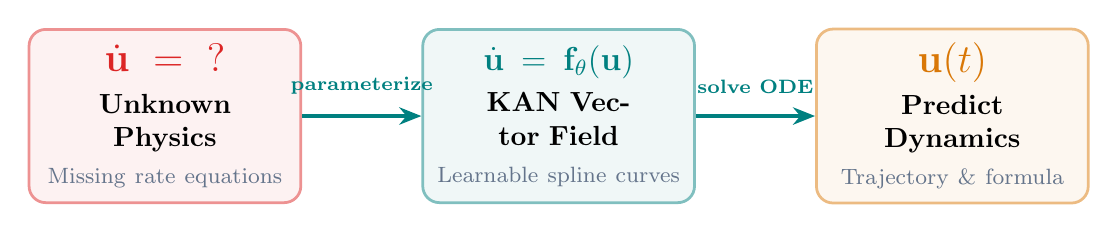
\begin{tikzpicture}[
    box/.style={
      rounded corners=6pt,
      minimum width=3.4cm,
      minimum height=2.2cm,
      text width=3.1cm,
      align=center,
      line width=1pt,
      inner sep=5pt
    },
    arrow/.style={
      -{Stealth[length=2.8mm,width=2.2mm]},
      line width=1.4pt,
      draw=KanTeal
    }]

    % 3 Main Flowchart Boxes (Spaced at 0, 5.0, 10.0 for 1.6cm clear arrow gap)
    \node[box,draw=KanRed!50,fill=KanRed!6] (box1) at (0,0) {
      {\Large\bfseries\color{KanRed} $\dot{\mathbf{u}} = {?}$}\\[0.3em]
      \textbf{Unknown Physics}\\[0.15em]
      {\footnotesize\color{KanSlate} Missing rate equations}
    };

    \node[box,draw=KanTeal!50,fill=KanTeal!6] (box2) at (5.0,0) {
      {\large\bfseries\color{KanTeal} $\dot{\mathbf{u}} = \mathbf{f}_{\theta}(\mathbf{u})$}\\[0.3em]
      \textbf{KAN Vector Field}\\[0.15em]
      {\footnotesize\color{KanSlate} Learnable spline curves}
    };

    \node[box,draw=KanGold!50,fill=KanGold!6] (box3) at (10.0,0) {
      {\Large\bfseries\color{KanGold} $\mathbf{u}(t)$}\\[0.3em]
      \textbf{Predict Dynamics}\\[0.15em]
      {\footnotesize\color{KanSlate} Trajectory \& formula}
    };

    % Clean flow arrows with labels directly on the path with upward offset
    \draw[arrow] (box1.east) -- node[above=4pt, font=\scriptsize\bfseries\color{KanTeal}] {parameterize} (box2.west);
    \draw[arrow] (box2.east) -- node[above=4pt, font=\scriptsize\bfseries\color{KanTeal}] {solve ODE} (box3.west);
  \end{tikzpicture}
  \end{center}

  \vspace{0.8em}
  \begin{columns}[T,onlytextwidth]
    \column{0.65\textwidth}
      \begin{beamercolorbox}[rounded=true,sep=0.55em]{block body}
        \scriptsize
        \textbf{Base Paper:} Z. Koenig, J. Kim, Y. Deng, \emph{KAN-ODEs: Kolmogorov--Arnold Network Ordinary Differential Equations for Learning Dynamical Systems and Hidden Physics}, CMAME / arXiv:2407.04192 (2024), MIT.
      \end{beamercolorbox}
    \column{0.32\textwidth}
      \begin{beamercolorbox}[rounded=true,center,sep=0.6em]{block title}
        \alert{\textbf{\small Learning Dynamic System}}\\[0.15em]
        \textbf{\small Hidden Equation Explore }
      \end{beamercolorbox}
  \end{columns}
\end{frame}

% =============================================================================
% SLIDE 3: Base Paper's Method (Three Key Decisions)
% =============================================================================
\begin{frame}{Base Paper's Method: Three Key Decisions}
  \vspace{0.2em}
  \begin{center}
  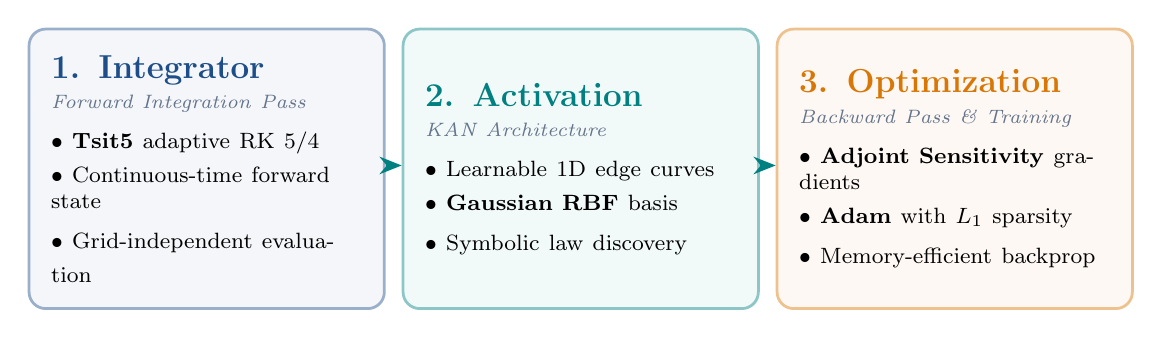
\begin{tikzpicture}[
    card/.style={
      rounded corners=6pt,
      minimum width=4.3cm,
      minimum height=3.55cm,
      text width=3.95cm,
      align=left,
      line width=1pt,
      inner sep=8pt,
      anchor=north west
    },
    arrow/.style={
      -{Stealth[length=2.8mm,width=2.2mm]},
      line width=1.4pt,
      draw=KanTeal
    }]

    % Card 1: Integrator
    \node[card,draw=KanBlue!45,fill=KanBlue!5] (c1) at (0,0) {
      {\bfseries\large\color{KanBlue} 1.\ \ Integrator}\\[-0.1em]
      {\scriptsize\itshape\color{KanSlate} Forward Integration Pass}\\[0.5em]
      \footnotesize
      $\bullet$ \textbf{Tsit5} adaptive RK 5/4\\[0.3em]
      $\bullet$ Continuous-time forward state\\[0.3em]
      $\bullet$ Grid-independent evaluation
    };

    % Card 2: Activation
    \node[card,draw=KanTeal!45,fill=KanTeal!5] (c2) at (4.75,0) {
      {\bfseries\large\color{KanTeal} 2.\ \ Activation}\\[-0.1em]
      {\scriptsize\itshape\color{KanSlate} KAN Architecture}\\[0.5em]
      \footnotesize
      $\bullet$ Learnable 1D edge curves\\[0.3em]
      $\bullet$ \textbf{Gaussian RBF} basis\\[0.3em]
      $\bullet$ Symbolic law discovery
    };

    % Card 3: Optimizer
    \node[card,draw=KanGold!45,fill=KanGold!5] (c3) at (9.5,0) {
      {\bfseries\large\color{KanGold} 3.\ \ Optimization}\\[-0.1em]
      {\scriptsize\itshape\color{KanSlate} Backward Pass \& Training}\\[0.5em]
      \footnotesize
      $\bullet$ \textbf{Adjoint Sensitivity} gradients\\[0.3em]
      $\bullet$ \textbf{Adam} with $L_1$ sparsity\\[0.3em]
      $\bullet$ Memory-efficient backprop
    };

    % Mathematically Guaranteed 100% Horizontal Connective Arrows
    \draw[arrow] ([yshift=-1.75cm]c1.north east) -- ([yshift=-1.75cm]c2.north west);
    \draw[arrow] ([yshift=-1.75cm]c2.north east) -- ([yshift=-1.75cm]c3.north west);
  \end{tikzpicture}
  \end{center}

  \vspace{0.45em}
  % Modern High-Impact Stat Highlight Card
  \begin{center}
  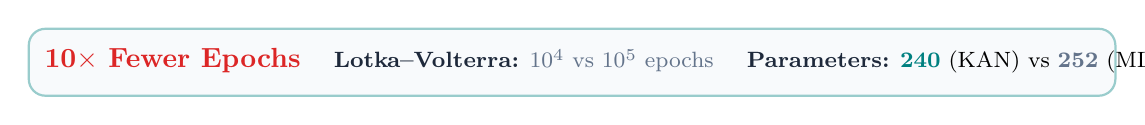
\begin{tikzpicture}
    \node[
      rounded corners=6pt,
      draw=KanTeal!40,
      fill=KanMist,
      line width=0.8pt,
      minimum width=13.8cm,
      minimum height=0.85cm,
      inner sep=4pt
    ] {
      \begin{minipage}{13.4cm}
        \centering\footnotesize
        \begin{tabular*}{\textwidth}{@{\extracolsep{\fill}} c c c @{}}
          \textbf{\color{KanRed}\normalsize 10$\boldsymbol{\times}$ Fewer Epochs} &
          \textbf{\color{KanInk}Lotka--Volterra:} {\color{KanSlate}$10^4$ vs $10^5$ epochs} &
          \textbf{\color{KanInk}Parameters:} {\color{KanTeal}\textbf{240}} (KAN) vs {\color{KanSlate}\textbf{252}} (MLP)
        \end{tabular*}
      \end{minipage}
    };
  \end{tikzpicture}
  \end{center}
\end{frame}

% =============================================================================
% SLIDE 4: Our Extensions (Structured 3-Card Comparison)
% =============================================================================
\begin{frame}{Our Extension: Stress-Testing the Design Choices}
  \vspace{0.1em}
  \centering
  {\footnotesize The base paper fixed \alert{\textbf{Tsit5 + Gaussian RBF}}. We systematically interrogate both choices.}

  \vspace{0.4em}
  \begin{center}
  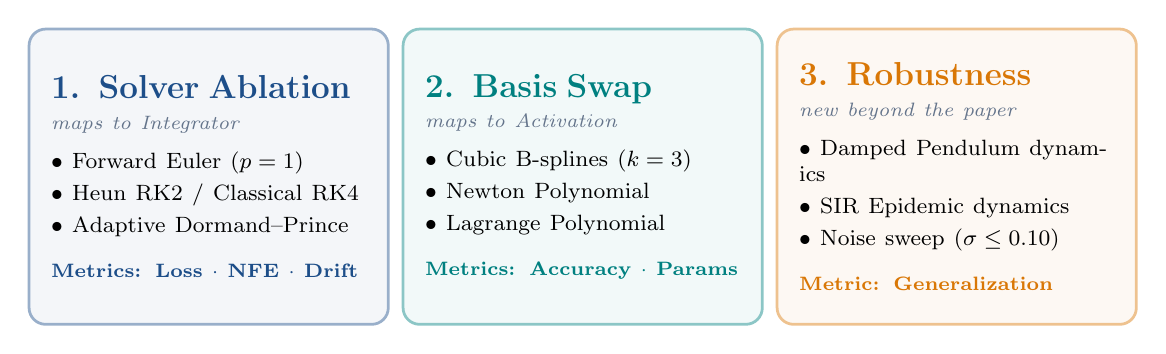
\begin{tikzpicture}[
    extcard/.style={
      rounded corners=6pt,
      minimum width=4.3cm,
      minimum height=3.75cm,
      text width=4.0cm,
      align=left,
      line width=1pt,
      inner sep=8pt,
      anchor=north west
    }]

    % Card 1: Solver Ablation
    \node[extcard,draw=KanBlue!45,fill=KanBlue!5] (e1) at (0,0) {
      {\bfseries\large\color{KanBlue} 1.\ \ Solver Ablation}\\[-0.1em]
      {\scriptsize\itshape\color{KanSlate} maps to Integrator}\\[0.45em]
      \footnotesize
      $\bullet$ Forward Euler ($p=1$)\\[0.25em]
      $\bullet$ Heun RK2 / Classical RK4\\[0.25em]
      $\bullet$ Adaptive Dormand--Prince\\[0.5em]
      \raggedright{\scriptsize\bfseries\color{KanBlue} Metrics: Loss $\cdot$ NFE $\cdot$ Drift}
    };

    % Card 2: Basis Swap
    \node[extcard,draw=KanTeal!45,fill=KanTeal!5] (e2) at (4.75,0) {
      {\bfseries\large\color{KanTeal} 2.\ \ Basis Swap}\\[-0.1em]
      {\scriptsize\itshape\color{KanSlate} maps to Activation}\\[0.45em]
      \footnotesize
      $\bullet$ Cubic B-splines ($k=3$)\\[0.25em]
      $\bullet$ Newton Polynomial \\[0.25em]
      $\bullet$ Lagrange Polynomial \\[0.5em]
      \raggedright{\scriptsize\bfseries\color{KanTeal} Metrics: Accuracy $\cdot$ Params}
    };

    % Card 3: Robustness
    \node[extcard,draw=KanGold!45,fill=KanGold!5] (e3) at (9.5,0) {
      {\bfseries\large\color{KanGold} 3.\ \ Robustness}\\[-0.1em]
      {\scriptsize\itshape\color{KanSlate} new beyond the paper}\\[0.45em]
      \footnotesize
      $\bullet$ Damped Pendulum dynamics\\[0.25em]
      $\bullet$ SIR Epidemic dynamics\\[0.25em]
      $\bullet$ Noise sweep ($\sigma \le 0.10$)\\[0.5em]
      \raggedright{\scriptsize\bfseries\color{KanGold} Metric: Generalization}
    };
  \end{tikzpicture}
  \end{center}

  \vspace{0.45em}
  \centering
  \scriptsize\textbf{Controlled Setup:} Adjoint gradients and Adam optimizer remain fixed, strictly isolating solver and basis effects.
\end{frame}

% =============================================================================
% SLIDE 5: Expected Methodology (Clean 4-Stage Pipeline + Results Matrix)
% =============================================================================
\begin{frame}{Expected Methodology: One Reproducible Pipeline}
  \vspace{0.2em}
  \begin{center}
  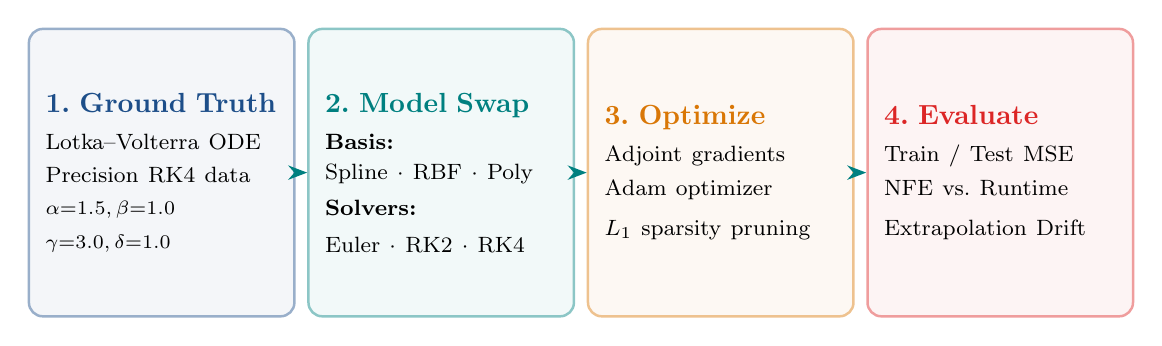
\begin{tikzpicture}[
    stepcard/.style={
      rounded corners=5pt,
      minimum width=3.2cm,
      minimum height=3.65cm,
      text width=2.95cm,
      align=left,
      line width=0.9pt,
      inner sep=6pt,
      anchor=north west
    },
    arrow/.style={
      -{Stealth[length=2.4mm,width=1.8mm]},
      line width=1.3pt,
      draw=KanTeal
    }]

    % Stage 1
    \node[stepcard,draw=KanBlue!45,fill=KanBlue!5] (s1) at (0,0) {
      {\bfseries\normalsize\color{KanBlue} 1.\ Ground Truth}\\[0.4em]
      \footnotesize
      Lotka--Volterra ODE\\[0.25em]
      Precision RK4 data\\[0.45em]
      {\scriptsize $\alpha{=}1.5, \beta{=}1.0$\\$\gamma{=}3.0, \delta{=}1.0$}
    };

    % Stage 2
    \node[stepcard,draw=KanTeal!45,fill=KanTeal!5] (s2) at (3.55,0) {
      {\bfseries\normalsize\color{KanTeal} 2.\ Model Swap}\\[0.4em]
      \footnotesize
      \textbf{Basis:}\\[0.15em]
      Spline $\cdot$ RBF $\cdot$ Poly\\[0.4em]
      \textbf{Solvers:}\\[0.15em]
      Euler $\cdot$ RK2 $\cdot$ RK4
    };

    % Stage 3
    \node[stepcard,draw=KanGold!45,fill=KanGold!5] (s3) at (7.1,0) {
      {\bfseries\normalsize\color{KanGold} 3.\ Optimize}\\[0.4em]
      \footnotesize
      Adjoint gradients\\[0.3em]
      Adam optimizer\\[0.3em]
      $L_1$ sparsity pruning
    };

    % Stage 4
    \node[stepcard,draw=KanRed!45,fill=KanRed!5] (s4) at (10.65,0) {
      {\bfseries\normalsize\color{KanRed} 4.\ Evaluate}\\[0.4em]
      \footnotesize
      Train / Test MSE\\[0.3em]
      NFE vs.\ Runtime\\[0.3em]
      Extrapolation Drift
    };

    % Connective arrows
    \draw[arrow] (s1.east) -- (s2.west);
    \draw[arrow] (s2.east) -- (s3.west);
    \draw[arrow] (s3.east) -- (s4.west);
  \end{tikzpicture}
  \end{center}

  \vspace{0.55em}
  \begin{columns}[T,onlytextwidth]
    \column{0.55\textwidth}
      \begin{beamercolorbox}[rounded=true,sep=0.45em]{block title}
        \scriptsize\textbf{Results Deliverable:}\\[0.15em]
        $\bullet$ Train/Extrapolation MSE \ $\cdot$\ NFE per step\\
        $\bullet$ Sensitivity to noise ($\sigma \le 0.1$) \ $\cdot$\ Wall-clock speed
      \end{beamercolorbox}
    \column{0.43\textwidth}
      \begin{beamercolorbox}[rounded=true,sep=0.45em]{block body}
        \scriptsize\textbf{Numerical Techniques Explore:}\\[0.15em]
        Euler/RK ODE integration \ $\cdot$\ Spline \& polynomial interpolation \ $\cdot$\ Truncation error \ $\cdot$\ Optimization
      \end{beamercolorbox}
  \end{columns}
\end{frame}

\end{document}